\documentclass[12pt,letterpaper]{hmcpset}
\usepackage[margin=1in]{geometry}
\usepackage{graphicx}

% info for header block in upper right hand corner
\name{Marc Laugharn}
\class{MATH189 - Math of Big Data}
\assignment{Midterm Project Writeup}

\begin{document}

%\tableofcontents

\section{Abstract}
My project was based on the Kaggle Deepfake Detection Challenge competition. 
I trained a convolutional neural network to discriminate between real and fake videos.
I used transfer learning on a pretrained resnet-18 model to speed up the training, and used data augmentation to generate synthetic examples to extend the relatively small number of examples.
I also used heatmaps to identify problems with the network and to improve its training.

\section{Introduction}
I trained a convolutional neural network to classify videos from a dataset containing both real and fake videos. 

\section{Dataset}
The dataset consisted of just over 470 GB of video footage.
Each video was 10 seconds long.
Both the training set and test contained 400 videos.
Each video in the training set is labeled either `real' or `fake'.
A video could be fake either due to forged video or forged audio.
I focused on detecting forged video, as it seemed more straightforward to me.

I split the training set videos into a smaller training set and a validation set at random, with a 70:30 split.

Because the dataset was so large, I hosted it all on Google Drive, which I was able to access through Google Colab notebooks.

\section{Preprocessing}
The videos were originally 1920x1080 pixels.
For the sake of GPU memory, the videos were resized to 1280x720 pixels.
The video was converted into images of the still frames.
The frames were sampled at 1 frame per second of video.
The dataset was loaded into batches of size 64, and then each channel of each image was normalized to match the mean and the variance of the RGB channels of images in the ImageNet dataset.

There were more fake examples than real examples, which could have lead to the model becoming more biased towards predicting `fake' by default.
I re-weighed the samples so that fake and real examples were sampled equally.
This came at the cost of reducing the variance of the real examples, but made the accuracy more representative of the model's classification ability.

\section{Data augmentation}
I applied numerous visual augmentations to sampled videos before they were observed by the network.
I anticipated this would make it more robust to minor visual changes.
The augmentations were:

\begin{itemize}
    \item Blur
    \item Median Blur
    \item Flip Left-Right
    \item Minor HSV color shift
    \item Crop and Pad
    \item Rotate
    \item Zoom
    \item Brightness change
    \item Contrast change
    \item Jpeg Compression
\end{itemize}
Each augmentation was applied with an associated probability.

\begin{figure}
    \centering
    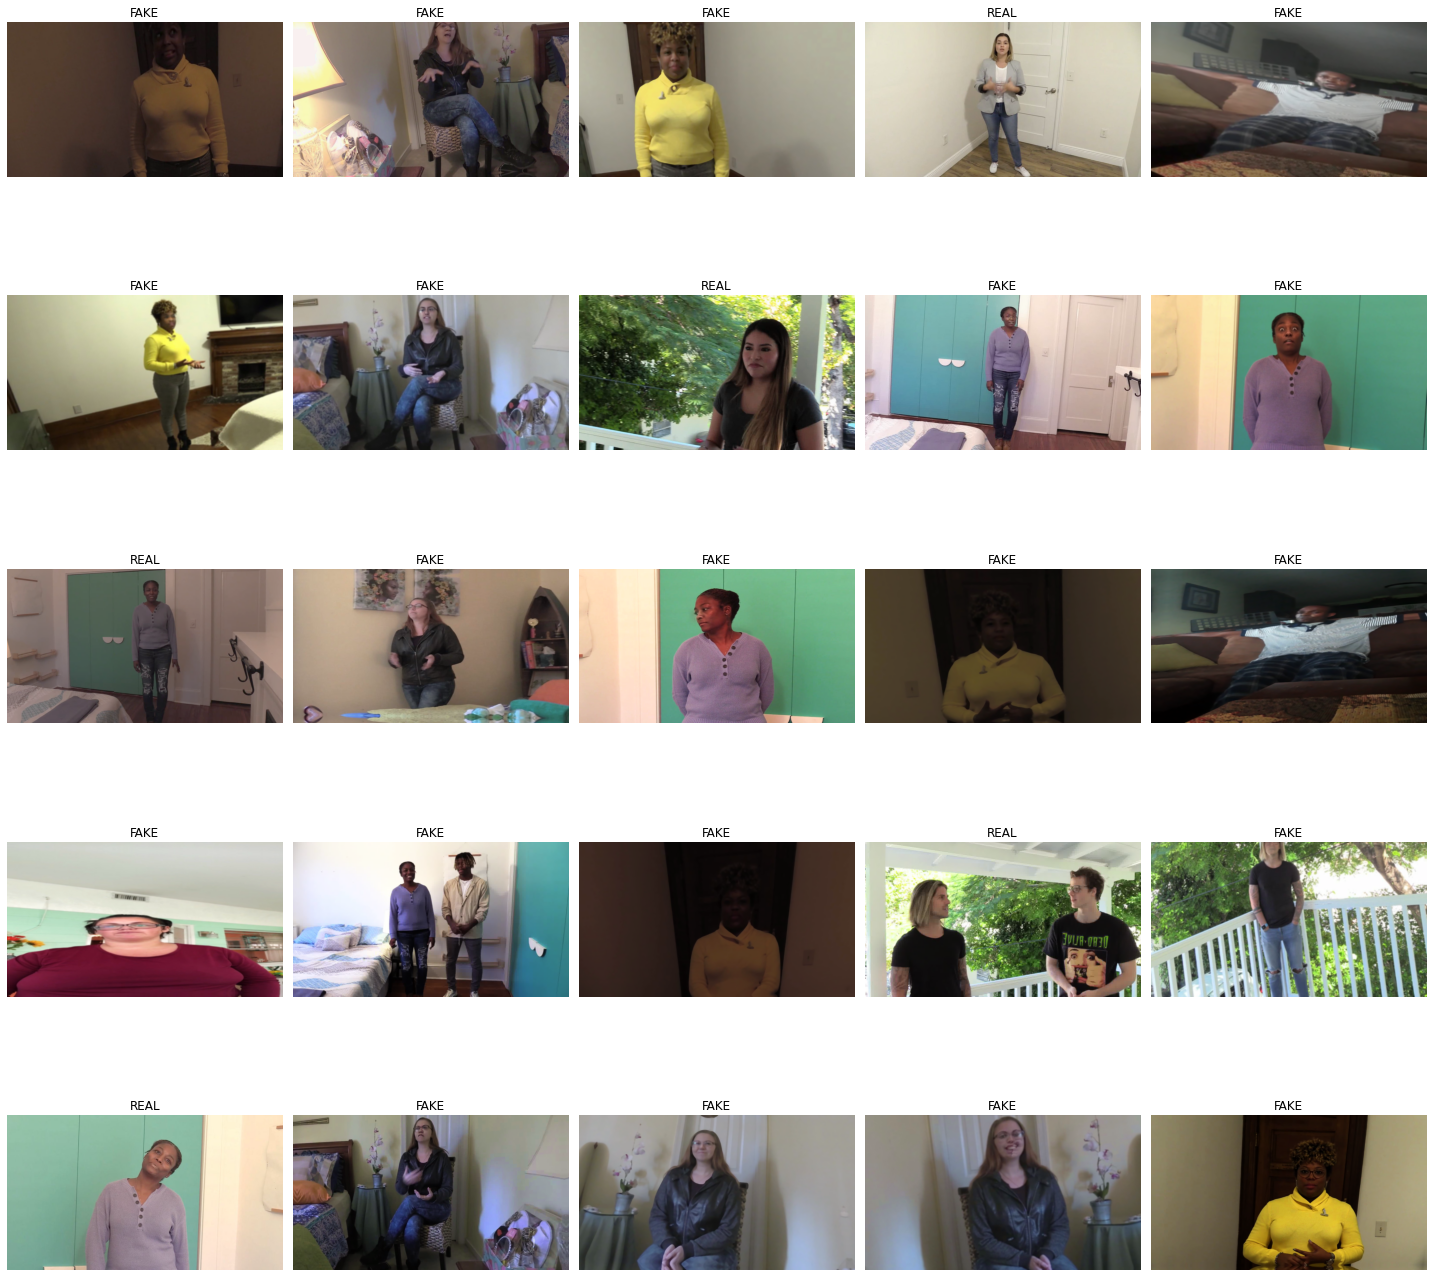
\includegraphics[width=\textwidth]{transformed}
    \caption{An example batch of images after being augmented}
\end{figure}

\section{Network architecture, training methods, and transfer learning}
I used a resnet-18 architecture for this problem, and used pre-trained weights to speed up the training portion of the task. 
I had previously seen that transfer learning using ResNets worked well for object recognition tasks, and was curious to see if it would work well with this problem. 

The pre-trained resnet-18 model had been trained to recognize objects according to the ImageNet dataset.
The ImageNet dataset consists of 1000 different objects seen across very different contexts, and quite different from the task at hand, but I assumed that a lot of the pre-trained weights from earlier layers would still be quite useful for this problem also.

I planned on using the pretrained resnet by altering mainly the later layers in the network to gear them towards the objective of detecting deepfake faces.
I figured because it was a deep neural network trained to recognize a wide variety of objects, its earliest layer were probably good at being general-purpose feature recognizers across a variety of tasks.\
fast.ai lets you do this by `freezing' the network - fixing the early layer groups so that they do not update with training.
Only the later layers update in a frozen network

fast.ai's deep learning library has a function that plots loss vs learning rate, which I used to determine a good learning rate for the model initially.

\begin{figure}
    \centering
    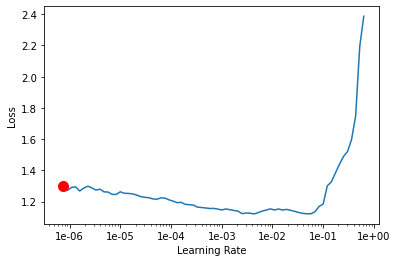
\includegraphics[width=\textwidth]{lossvlearningrate}
    \caption{Result of find\_lr(), plotting the loss vs the learning rate}
\end{figure}
    I used lower learning rates for the earlier layers and higher training rates for the later layers, because I imagined it would be more useful to update the last layers more than the first layers.

I used a one-cycle learning rate schedule with an Adam optimizer.
Cyclic learning rate schedules start off with a low learning rate initially, increasing over the course of the epochs to help escape local minima, and then finally decreases again towards the end of the schedule.
This hopefully trained it faster.
Adam is an adaptive learning rate optimizer that behaves like stochastic gradient descent with varying momentum.

I trained in numerous sets of epochs.
\begin{itemize}
    \item 5 epochs, learning rate = slice(2e-4, 1e-2)
    \item 3 epochs, learning rate = slice(2e-4, 2e-2)
    \item 3 epochs, frozen network, learning rate = 1e-2
\end{itemize}

\begin{figure}
    \centering
    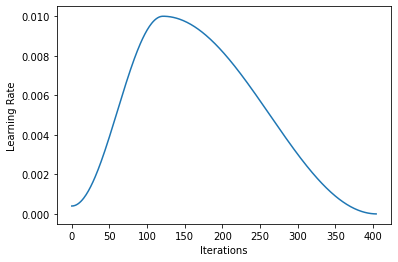
\includegraphics[width=\textwidth]{cycliclr}
    \caption{The learning rate over the course of the first 5 epochs, showing the shape of a cyclic learning rate schedule}
\end{figure}

\begin{figure}
    \centering
    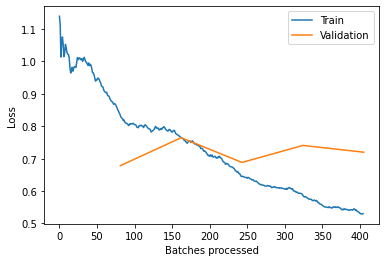
\includegraphics[width=0.3\textwidth]{loss1}
    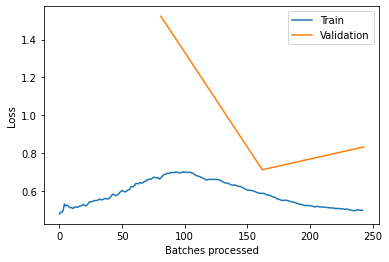
\includegraphics[width=0.3\textwidth]{loss2}
    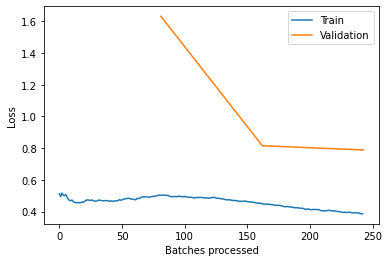
\includegraphics[width=0.3\textwidth]{loss3}
    \caption{The loss plot for the first 5 epochs [left], the next 3 epochs [middle], and the last 3 epochs with the network frozen [right]}
\end{figure}
\section{Evaluation and interpretation}
\begin{figure}
    \includegraphics[width=\textwidth]{toplosses}
    \caption{The images with the worst predictions}
\end{figure}
\begin{figure}
    %\includegraphics[width=\textwidth]{toplossesheatmap}
    \caption{The heatmaps of images with the worst predictions}
\end{figure}
\begin{figure}
    %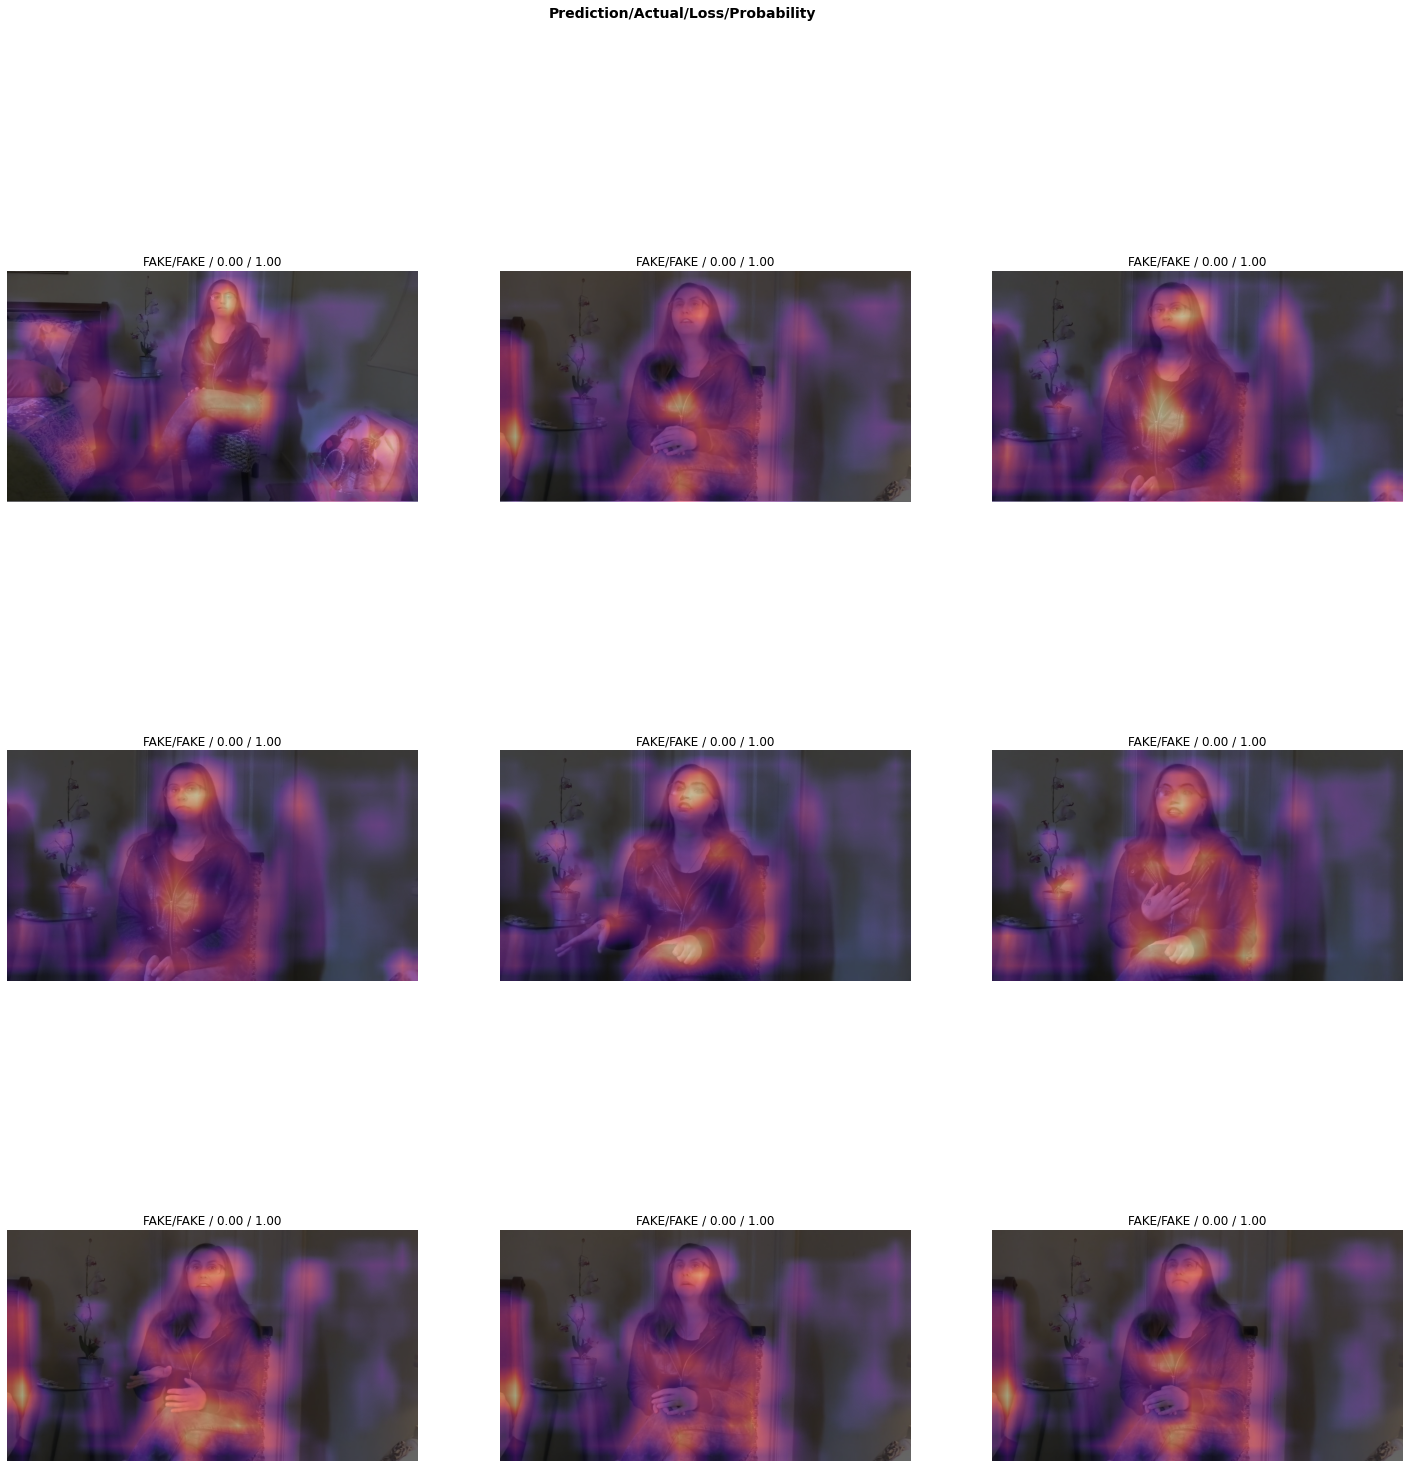
\includegraphics[wdith=\textwidth]{lowlossheatmap}
    \catpion{The heatmaps of images with the best predictions}
\end{figure}
Because this is a classification problem I used a cross-entropy loss function.
During each epoch I measured training loss, validation loss, and accuracy.

I was able to reach 75\% accuracy.

I used Gradient-Class Activated Mapping (Grad-CAM) heatmaps to produce visual explanations of the decisions made by the CNN based on the gradients flowing into the last layer from each pixel.

On the images with the best measured loss, they often were most confident due to the face regions of fake videos. On images with the worst loss, the network was often confused and weighed its classifications strongly of non-face objects.

In the worst loss examples, there is actually a man wearing a t-shirt that has a face on it, which probably also confused the model.

It also seems as though the resnet was still quite strongly suited towards recognizing objects, rather than detecting fake faces.

\section{Further improvements}
\begin{itemize}
    \item For the sake of training speed, I opted to use a resnet-18 model, but a resnet-32 or resnet-50 model (with 32 or 50 residual block layers, as opposed to 18) would probably do better. 
I think it would also be wise to train for many more epochs.

    \item It may also be prudent to use a different base model to train from, as a resnet may be too specific to object recognition for this task.

    \item I would also incorporate a lot more external examples of fake faces, such as the FaceForensics++ dataset.

    \item It would also make sense to crop the frames to the face region (including a large surrounding margin), as the model is spending a lot of time looking for useful information in regions far away from faces.

    \item I would also use an ensemble of classifiers to reduce the variance of the model, and if possible I would do a test for synthetic audio by analyzing bispectral artifacts of synthesis that are unlikely to be produced by real human vocal chords.

    \item Also, As Prof Gu suggested, it would also be prudent to sample the frames of the videos according to how useful an example it is for the task of discriminating between `real' and `fake' as opposed to uniformly sampling them.

\end{itemize}


% Add pairs of problems and solutions as needed

\end{document}
